\documentclass{standalone}
\usepackage{tikz}
\usepackage{tabularx}
\usepackage{colortbl}
\usepackage{booktabs}

\begin{document}
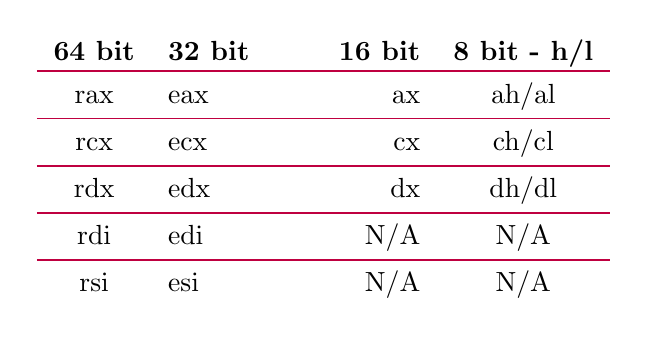
\begin{tikzpicture}

\node (tbl) {
\begin{tabularx}{.6\textwidth}{cXrcc}
\arrayrulecolor{purple}
\textbf{64 bit} & \textbf{32 bit} & \textbf{16 bit} & \textbf{8 bit - h/l} \\
\toprule
rax & eax & ax & ah/al \\ 
\midrule
rcx & ecx & cx & ch/cl  \\
\midrule
rdx & edx & dx & dh/dl \\ 
\midrule
rdi & edi & N/A & N/A \\
\midrule
rsi & esi & N/A & N/A
\end{tabularx}
};

\end{tikzpicture}
\end{document}